\subsubsection*{Caso 2: TRAVE CON 2 APPOGGI}
$||\bar{R}_1 + \bar{R}_2|| = ||\bar{P}|| \Rightarrow \Sigma \bar{F} = \bar{R}_1 + \bar{R}_2 + \bar{P} = 0 \Rightarrow a_{CM} = 0$
affinché il corpo rimanga in equilibrio, quanto valgono $||\bar{R}_1||$, $||\bar{R}_2||$?
$R_1, R_2$ dipendono da $x$?
c'è un caso in cui il corpo non è mai in equilibrio?

\begin{figure}[H]
\raggedleft
\begin{tikzpicture}
% trave
\draw[thick] (2, 0) rectangle (4, 0.4);
% appoggi
\filldraw[green] (2.2, 0) -- (2.0, -0.4) -- (2.4, -0.4) cycle;
\node[below] at (2.2, -0.4) {1};
\filldraw[green] (3.6, 0) -- (3.4, -0.4) -- (3.8, -0.4) cycle;
\node[below] at (3.6, -0.4) {2};
% forze
\draw[->] (2.2, 0.4) -- (2.2, 1) node[above] {$R_1$};
\draw[->] (3.6, 0.4) -- (3.6, 1) node[above] {$R_2$};
\filldraw (3, 0.2) circle (1pt) node[above] {$CM$};
\draw[->] (3, 0) -- (3, -0.8) node[below] {$P$};
% quote
\draw[<->] (2.2, -0.2) -- (3, -0.2) node[midway, below] {$L/2$};
\draw[<->] (3, 0.2) -- (3.6, 0.2) node[midway, above] {$x$};
% assi
\draw[->] (4.5, 0.5) -- (5, 0.5) node[right] {$\hat{x}$};
\draw[->] (4.5, 0.5) -- (4.5, 1) node[above] {$\hat{y}$};
\draw[->] (4.5, 0.5) circle (2pt);
\node at (4.8, 0.2) {$\hat{z}$};
\end{tikzpicture}
\end{figure}

$$ \Sigma \bar{\tau}_{CM} = 0 = -\frac{L}{2} \hat{x} \times \bar{R}_1 + 0 \times \bar{P} + x \hat{x} \times \bar{R}_2 = -\frac{R_1 L}{2} (\hat{x} \times \hat{y}) + x R_2 (\hat{x} \times \hat{y}) = 0 $$
$$ \begin{cases}
R_1 + R_2 = P \\
x R_2 = R_1 L/2
\end{cases} \Rightarrow R_1 = Mg \left( \frac{2x}{2x+L} \right) \quad R_2 = Mg \left( \frac{L}{2x+L} \right) $$

$\Rightarrow R_1, R_2 \ge 0$ pk il corpo è in equilibrio
$\Rightarrow R_1 \ge 0$ solo se $x \ge 0$
$\Rightarrow$ in generale $R_2 \ge 0$ sempre e $-L/2 < x \le L/2$
Quindi il corpo è in equilibrio solo se $x \ge 0$.
Se $x < 0$ il corpo non è in equilibrio e ruota intorno al perno 2.

* trave con 3 appoggi. nel mondo reale i corpi completamente rigidi non esistono, tendono a piegarsi su loro stessi infatti solitamente una trave ha 2 perni alle estremità e uno al centro.

\subsubsection*{Caso 3: CORPO IN PURO ROTOLAMENTO SUL PIANO ORIZZONTALE}
\begin{figure}[H]
\raggedleft
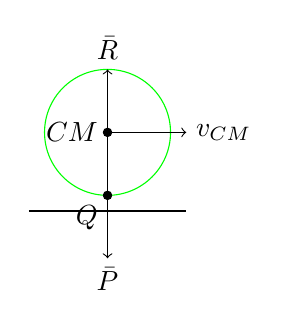
\begin{tikzpicture}
% piano
\draw[thick] (2, 0) -- (4, 0);
% corpo
\draw[green] (3, 1) circle (0.8cm);
\filldraw (3, 1) circle (1.5pt) node[left] {$CM$};
\draw[->] (3, 1) -- (4, 1) node[right] {$v_{CM}$};
% forze
\filldraw (3, 0.2) circle (1.5pt) node[below left] {$Q$};
\draw[->] (3, 0.2) -- (3, -0.6) node[below] {$\bar{P}$};
\draw[->] (3, 0.2) -- (3, 1.8) node[above] {$\bar{R}$};
\end{tikzpicture}
\end{figure}

$||\bar{R}|| = ||\bar{P}|| \Rightarrow \Sigma \bar{F} = \bar{R} + \bar{P} = 0 \Rightarrow a_{CM} = 0$ (quota fissa)
$||F_{S}|| = ||\Sigma \bar{F}_{\parallel \text{ al piano}}|| = 0$ quindi $\Sigma \bar{F}_{EXT} = 0$ \checkmark

Poiché Q è istantaneamente fermo potrebbe esserci attrito per mantenere il puro rotolamento (ex. piano inclinato) ma in questo caso non ci sono Forizzontali.
$\Sigma \bar{\tau}_{CM} = 0$ pk sia $\bar{P}$ che $\bar{R}$ passano per il centro CM, quindi la distanza fra polo e punto di applicazione è 0.

$\Rightarrow$ moto rettilineo uniforme e quiete = EQUILIBRIO PUNTO \\
moto di puro rotolamento e quiete = EQUILIBRIO CORPO

\subsection*{TENSORE D'INERZIA (o MATRICE D'INERZIA)}
un corpo è in pura rotazione intorno a $\hat{\omega}$
\begin{figure}[H]
\raggedleft
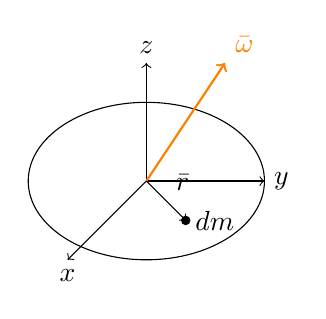
\begin{tikzpicture}
% corpo rigido
\draw (2, 1) ellipse (1.5cm and 1cm);
% assi
\draw[->] (2, 1) -- (2, 2.5) node[above] {$z$};
\draw[->] (2, 1) -- (3.5, 1) node[right] {$y$};
\draw[->] (2, 1) -- (1, 0) node[below] {$x$};
% omega
\draw[->, thick, orange] (2, 1) -- (3, 2.5) node[above right] {$\bar{\omega}$};
% vettore r
\draw[->] (2, 1) -- (2.5, 0.5) node[midway, above right] {$\bar{r}$};
\filldraw (2.5, 0.5) circle (1.5pt) node[right] {$dm$};
\end{tikzpicture}
\end{figure}

$$ \begin{cases}
\bar{r} = \hat{x}x + \hat{y}y + \hat{z}z \\
\bar{\omega} = \hat{x}\omega_x + \hat{y}\omega_y + \hat{z}\omega_z \\
\bar{L} = \hat{x}L_x + \hat{y}L_y + \hat{z}L_z
\end{cases} \Rightarrow \bar{L}_O = \int_{CR} dm \, \bar{r} \times (\underbrace{\bar{\omega} \times \bar{r}}_{= \bar{v}}) = \bar{L} $$
$ = (\bar{r} \cdot \bar{r})\bar{\omega} - (\bar{r} \cdot \bar{\omega})\bar{r} $

\begin{align*}
\bar{L} &= \int_{CR} dm \left[ (x^2+y^2+z^2)(\hat{x}\omega_x + \hat{y}\omega_y + \hat{z}\omega_z) - (x\omega_x + y\omega_y + z\omega_z)(\hat{x}x + \hat{y}y + \hat{z}z) \right] \\
&= \int_{CR} dm \left\{ \left[ (y^2+z^2)\omega_x - xy\omega_y - xz\omega_z \right]\hat{x} + \left[ (z^2+x^2)\omega_y - yx\omega_x - yz\omega_z \right]\hat{y} + \left[ (x^2+y^2)\omega_z - zx\omega_x - zy\omega_y \right]\hat{z} \right\} \\
&= \hat{x}L_x + \hat{y}L_y + \hat{z}L_z
\end{align*}

* in generale $\hat{x}, \hat{y}, \hat{z}$ non sono assi principali!
